\section{Introduction}
In this report, we will cover central topics of the Analysis, Design and Software Architecture course (BDSA) as we have applied them to our project during the Fall of 2012.\\
\newline
The report documents our activities ranging from our usage of the Rational Unified Process (RUP) artifacts \cite[p.~31]{OOAD} to our usage of the Scrum methodology to manage our agile development. Moreover, we will discuss several C\# technologies and how we have applied them to make our proof of concept.\\
\newline
After a brief introduction to Scrum, we have structured this document as a series of sprints (timeboxed periods of incremental development), each documenting our steps towards release date (the project delivery date). The report is structued this way to give a better view of the iterative process and show where in the process we have utilized the different software engineering tools and processes.\\
\newline
Because of the limited time we have to do the project we have decided to limit ourselves to the following three sprints:\\
\begin{itemize}
\item An introductory sprint, in which we focus a lot on major design and architectural decisions as well as programming some high-risk elements on our system
\item A longer, ‘elaboration’ sprint in which we focus on detailed design and analysis of major components as well as connecting important sub-systems 
\item Finally, a release sprint, in which we fine tuned selected components as well as made the adjustments to our documentation to make it a documentation of a product as well as a process.
\end{itemize}
In each sprint, we will describe the artifacts created in the sprint. However,
we would like to note two things relevant to the structure of our report:\\
\begin{enumerate}
\item The order of which the artifacts appear in the sprint is not necessarily equal to the
  order in which they were created (internally in the sprint). Each artifact
  may be created and revised several times during a sprint as it is relevant
  to the understanding of a design or a requirement. 
\item Not all reviews and revisions of the artifacts are described in the
  report. Only significant changes to an artifact or any change we find to have particular value will be highlighted.
\end{enumerate}
\subsection{Scrum}
As mentioned in the previous section, we will use the Scrum method to manage iterative development. Before we cover the actual sprints, we will present an overview of Scrum and the Scrum activities we will do the in sprints.
\newline
Scrum is an iterative framework designed to manage software development projects \cite{scrumguide} \\
The methods originally intends to include a team of up to eight persons, along with a Scrum Master and a Product Owner. However, as we were only five persons we had no choice but to appoint these roles to team members. Moreover, we decided that we wanted a more democratic approach to the features that we included in our project; this implied that the responsibility of creating product backlog items were spread out on the whole group instead of relying solely on the Product Owner \cite[p.~12]{scrumguide}.
\subsubsection{Daily Scrum}
According to the Scrum methodology, each full workday (in all sprints) is initiated with a daily Scrum. In this 15 minute meeting, we each report how progress is made with each task that is on the product backlog. Moreover, each team member can request help from other member in regards to difficult tasks. We use the Task Board of our Scrum tool as our primary form of task management. Each team member is standing up as to signal the immediate focus needed to do an effective meeting. In any case where a team member need some help, the Scrum Master either immediately facilitate the help needed (e.g declaring another members to a particular task) or he undertakes the responsibility to get the help needed later. Below is a picture a of a Scrum meeting with all members standing up around the Task Board, which is projected on a canvas.
\begin{figure}[H]
  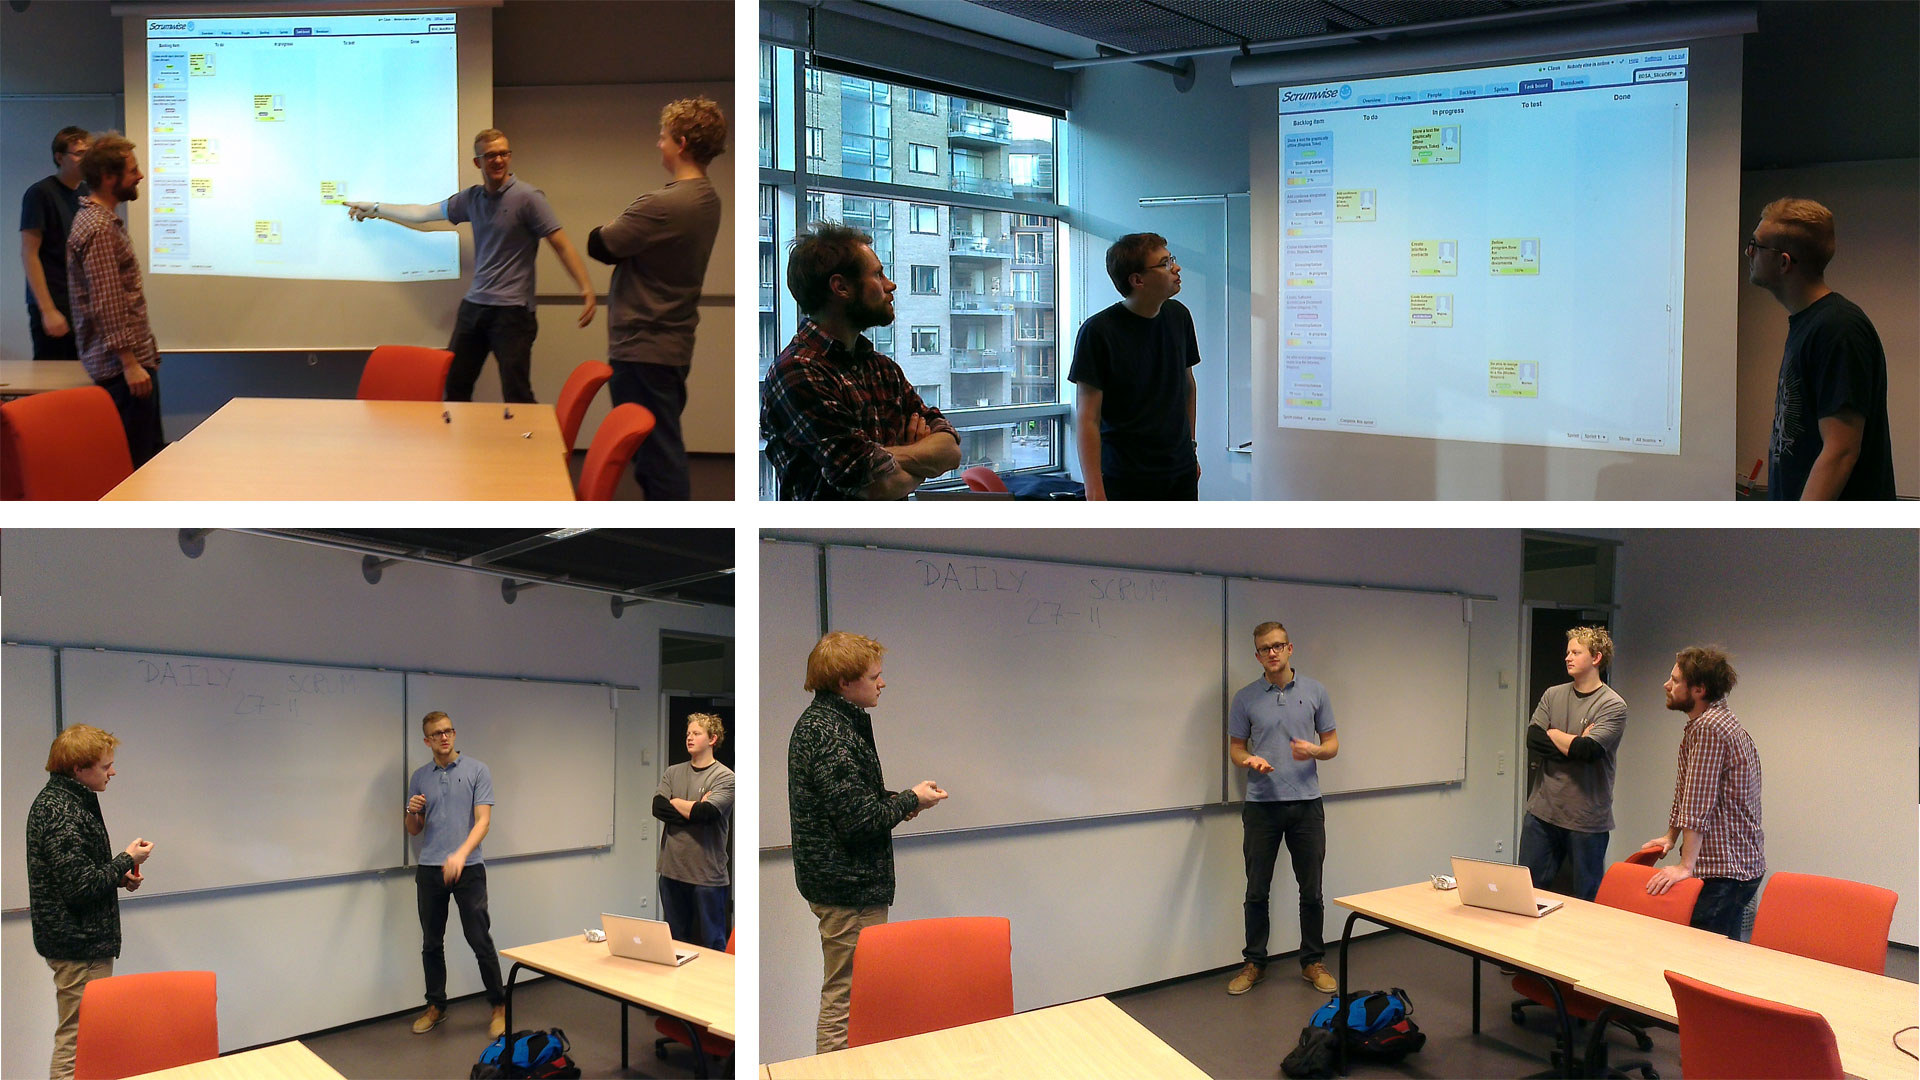
\includegraphics[width=\textwidth]{illustrations/DailyScrumCombined.jpg}
  \caption{Daily Scrum}
  \label{dailyscrum}
\end{figure}
\begin{figure}[H]
  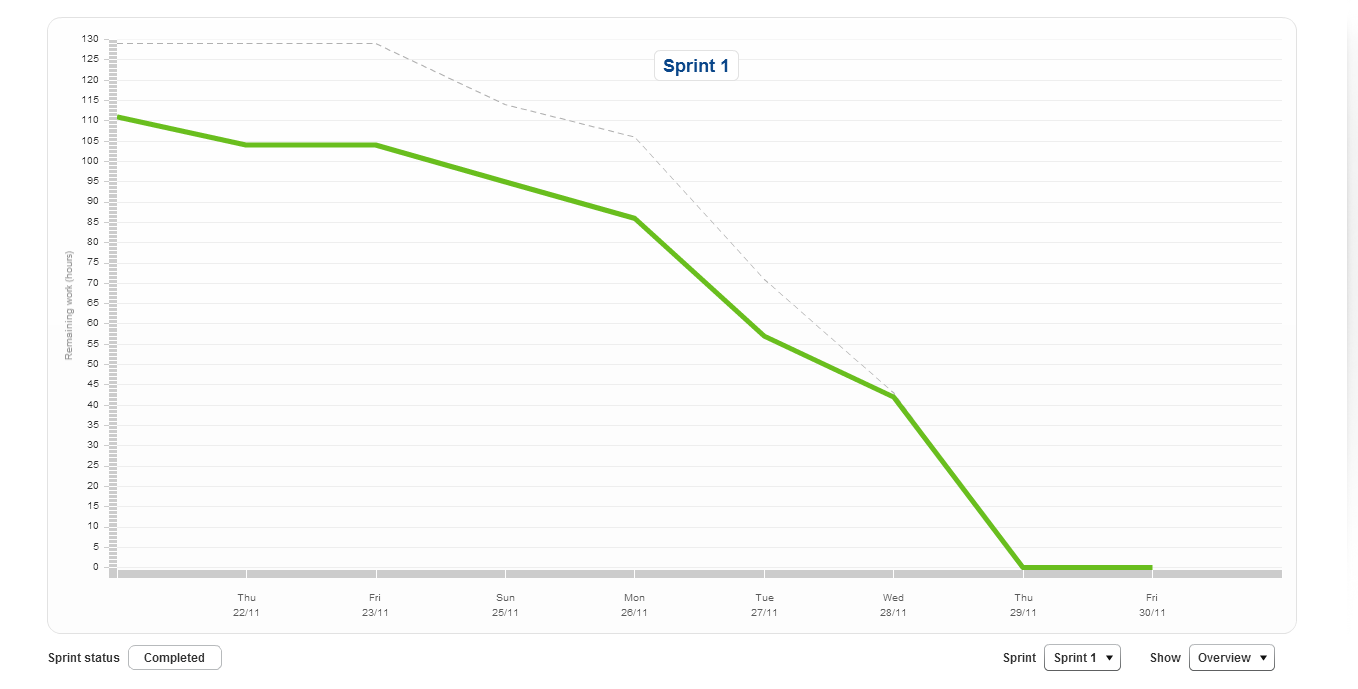
\includegraphics[width=\textwidth]{illustrations/burndown.png}
  \caption{Burndown chart}
  \label{burndown}
\end{figure}
After the Daily Scrum, the Scrum Master reviews the burndown chart for the sprint and compares it to the release date. 
\subsubsection{Sprint planning}
The Sprint planning meeting is the planning of the upcoming sprint. The different stories in the product backlog are prioritized. It is decided which tasks the sprint should consist of and the workload capacity of each team member is determined.
\subsubsection{Sprint review}
The review is the process of reviewing the work that has been done in the sprint, with focus on the the backlog items. The main goal of this activity is to measure the project against the goals determined in the sprint-planning.
\subsubsection{Sprint retrospective}
In conclusion of the scrum activities, we do a Scrum Retrospective. The retrospective mainly focuses on reviewing the process of doing Scrum, as opposed to the concrete backlog items. The main goal of this activity is to increase the productivity of each sprint iteratively by actively inspecting each Scrum related activity.